\apendice{Documentación técnica de programación}

\section{Introducción}
Este apéndice se centra en proporcionar una visión técnica detallada del desarrollo del proyecto. El objetivo es poder proporcionar una referencia a los futuros desarrolladores que requieran de la comprensión de la estructura del código y los procesos de compilación e instalación.

En las siguientes secciones se describen la organización de directorios del proyecto, un manual del programador con instrucciones para acceder al proyecto y sus respectivas configuraciones, y los procesos de configuración, instalación y ejecución del proyecto.

\section{Estructura de directorios}
A continuación se explican todos los directorios del \href{https://github.com/jpg1011/TFG-GestorTareasMoodle}{repositorio} del proyecto \cite{flutter_estructura}:

\begin{itemize}
    \item \textbf{app/app:} contiene todo el proyecto de Flutter. Se divide en las siguientes subcarpetas:
        \begin{itemize}
            \item \textbf{/android:} directorio generado por Flutter que contiene todos los archivos y carpetas necesarios para ejecutar la aplicación en dispositivos \textit{Android}.
            \item \textbf{/assets:} carpeta que contiene todo el contenido audiovisual de la aplicación, en este caso imágenes.
            \item \textbf{/ios:} directorio que contiene configuraciones, ejecutables, etc, que permiten ejecutar la aplicación en dispositivos \textit{iOS}.
            \item \textbf{/lib:} directorio que contiene todo el código fuente de la aplicación. Dentro de este directorio hay distintos subdirectorios, cada uno de ellos con una función:
            \begin{itemize}
                \item \textbf{/backend:} contiene el backend de cada una de las funcionalidades de la aplicación.
                \item \textbf{/config:} contiene ficheros de configuración de la aplicación.
                \item \textbf{/models:} contiene ficheros que representan cada uno de los modelos de la aplicación.
                \item \textbf{/presentation:} contiene todas las capas de presentación de \textit{UI}, dentro de esta carpeta se distinguen:
                    \begin{itemize}
                        \item \textbf{/screens:} representación de las pantallas de la aplicación, donde cada funcionalidad tiene su propio directorio.
                        \item \textbf{/widgets:} se dividen en directorios por cada funcionalidad, en cada directorio hay \textit{widgets} para mejorar la reutilización.
                    \end{itemize}
                \item \textbf{/services:} contiene el fichero que se encarga de comunicarse con la API de Moodle.
                \item \textbf{/utils:} contiene un fichero con elementos comunes en toda la aplicación.
            \end{itemize}
            \item \textbf{/linux:} directorio que contiene todo lo relacionado a configuraciones de \textit{Linux} para por ejecutar la aplicación en este entorno.
            \item \textbf{/macos:} directorio que contiene todo lo relacionado al sistema operativo de \textit{MacOS} para por ejecutar la aplicación en este entorno.
            \item \textbf{/windows:} este directorio contiene todos los archivos que permiten ejecutar la aplicación en \textit{Windows}.
        \end{itemize}
    \item \textbf{docs:} contiene todos los documentos \LaTeX 
\end{itemize}

\section{Manual del programador}
En esta sección se detallan todos los pasos a seguir para instalar y ejecutar localmente el proyecto correctamente.

\subsubsection{Configuración del entorno}
A continuación se explican todos los pasos a seguir para instalar el proyecto desde el repositorio de \textit{GitHub}.

Antes de instalar el proyecto en el equipo, es necesario tener instalado el editor de código Visual Studio Code, así como Git, posteriormente se indicarán las extensiones recomendables para el uso de \textit{Dart} y \textit{Flutter}.

Por otra parte, es necesario tener instalado en el equipo tanto \textit{Dart} como \textit{Flutter}. En este caso, no es necesario hacer una instalación directa de \textit{Dart}, ya que viene incluido en la instalación de \textit{Flutter}.

El primer paso es acceder a la \href{https://docs.flutter.dev/install/manual}{página de instalación de Flutter} y descargar el instalador del sistema que se esté utilizando. Se recomienda crear una carpeta para almacenar el \textit{SDK}. Se debe de extraer el \textit{SDK} del \textit{zip} en la carpeta creada. Por último, se crea una variable de entorno en el \textit{PATH} haciendo referencia a la ruta de la carpeta: \verb|<ruta_carpeta>\flutter\bin| \cite{flutter_instalacion}.

Para comprobar si la instalación se ha realizado con éxito, introduce el siguiente comando:
\begin{verbatim}
    flutter doctor
\end{verbatim}
Este comando realiza un diagnostico de la instalación y configuración del entorno. En caso de que falte algún elemento, se mostrará por pantalla y se deberá de proceder a su instalación.

Por otra parte, en Visual Studio Code se deben de instalar las extensiones \textit{Dart} y \textit{Flutter}, que permiten hacer uso de \textit{Dart} y \textit{Flutter}, ademas de facilitar el desarrollo al incluir atajos.

\subsubsection{Instalación del proyecto}

A continuación se procederá a la instalación del proyecto. Para ello, se debe de realizar una clonación del repositorio del proyecto. Para ello, se utiliza una terminal de comandos y se introducirá el siguiente comando:
\begin{verbatim}
git clone https://github.com/jpg1011/TFG-GestorTareasMoodle.git
\end{verbatim}

Posteriormente a la instalación del proyecto, se accederá a la carpeta de proyecto mediante el siguiente comando:
\begin{verbatim}
    cd TFG-GestorTareasMoodle/app/app
\end{verbatim}

Por último, ejecutar el siguiente comando, que abrirá el editor de código:
\begin{verbatim}
    code .
\end{verbatim}

\section{Compilación y ejecución del proyecto}
En esta sección se describen los pasos a seguir para compilar y ejecutar el proyecto. Se incluye una configuración del emulador para simular la aplicación en entornos Android.

\subsubsection{Configuración de simulador}
Para poder disponer de un emulador Android, primero es necesario instalar Android Studio, desde el cual se creará el emulador.

Una vez instalado Android Studio, se accede a la sección de emuladores desde el siguiente botón:
\begin{figure}[H]
    \centering
    
\includegraphics[width=0.7\linewidth]{img/boton_emulador.png}
    \caption{Botón de acceso a la configuración de emuladores}
    \label{fig:boton_emulador}
\end{figure}

Posteriormente, aparecerá la sección de emuladores y se debe de presionar el siguiente botón para añadir un nuevo emulador.
\begin{figure}[H]
    \centering
    \includegraphics[width=0.7\linewidth]{img/añadir_emulador.png}
    \caption{Botón para añadir nuevos emuladores}
    \label{fig:añadir_emulador}
\end{figure}

Una vez presionado el botón (imagen \ref{fig:añadir_emulador}), se selecciona la opción \textit{Create Virtual Device}.

A continuación, aparecerá una ventana con todas las imágenes de sistema disponibles para instalar en el emulador. Se seleccionará la siguiente imagen:
\begin{figure}[H]
    \centering
    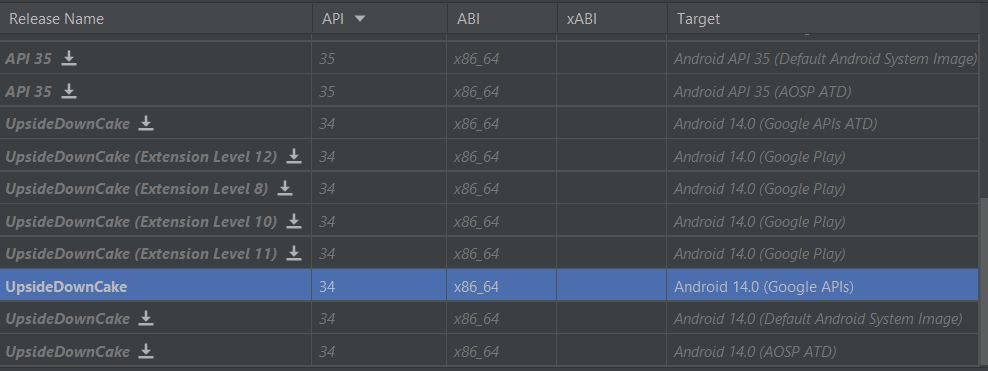
\includegraphics[width=0.7\linewidth]{img/system_image.png}
    \caption{Ventana con imágenes del sistema}
    \label{fig:system_images}
\end{figure}

Por último, aparecerá una pantalla de configuraciones generales del emulador. En este caso, se dejará todo de la misma forma.
\begin{figure}[H]
    \centering
    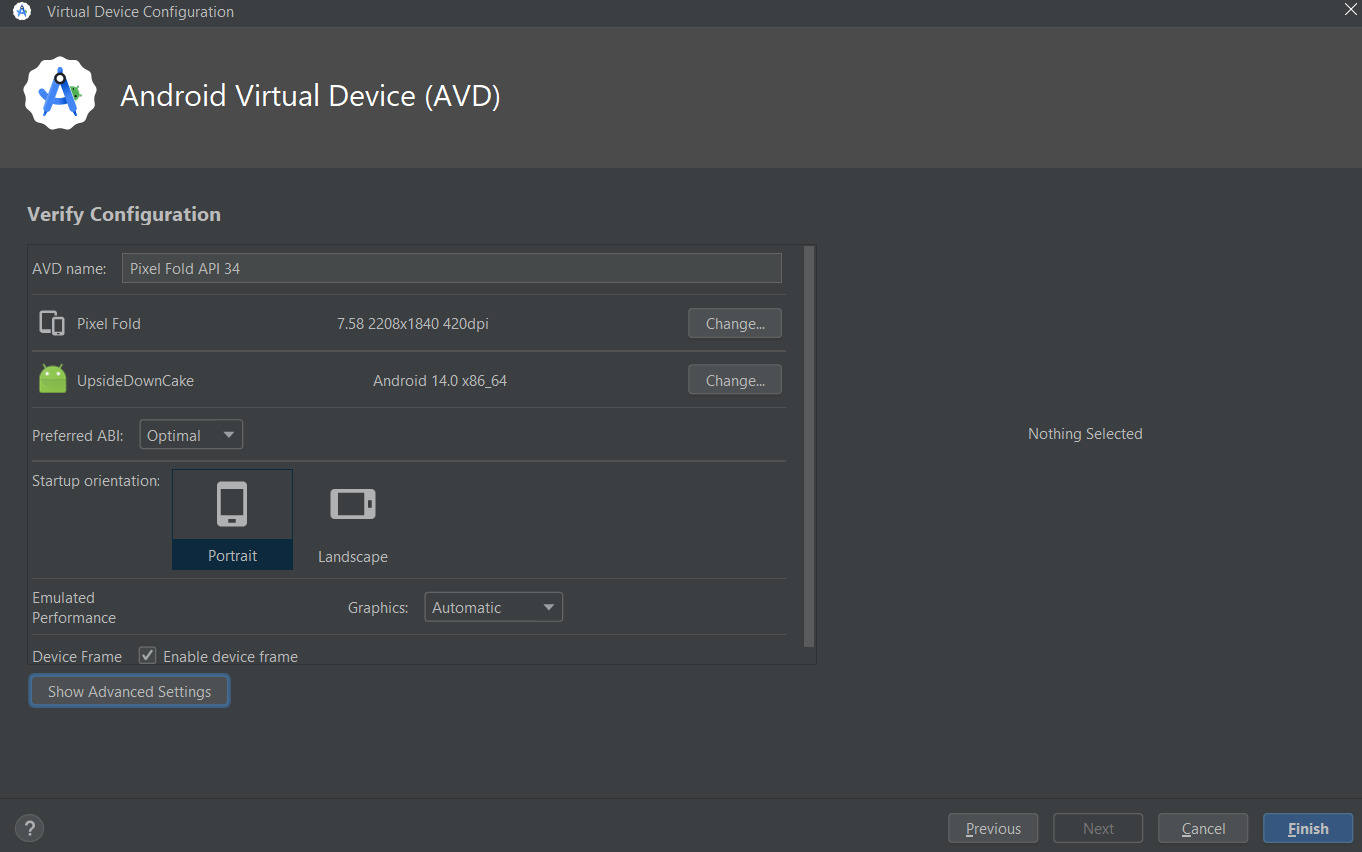
\includegraphics[width=0.9\linewidth]{img/pantalla_final_emulador.png}
    \caption{Ventana de configuración general del emulador}
    \label{fig:pantalla_final_emulador}
\end{figure}

\subsubsection{Instalación de dependencias}
Para poder ejecutar la aplicación es necesario tener instaladas las dependencias requeridas por la aplicación.

Para ello, será necesario ejecutar por terminal el siguiente comando:
\begin{verbatim}
    flutter pub get
\end{verbatim}

Tras la instalación de las dependencias se puede proceder con la ejecución de la aplicación.

\subsubsection{Ejecución de la aplicación}
A continuación se detallan los pasos necesarios para poder ejecutar la aplicación en el emulador instalador previamente.
El primer paso es pulsar la combinación de teclas \verb|Ctrl + Shift + P|. Se mostrará una ventana con un campo de texto en el que hay que introducir: \textit{Flutter: Launch Emulator}.
\begin{figure}[H]
    \centering
    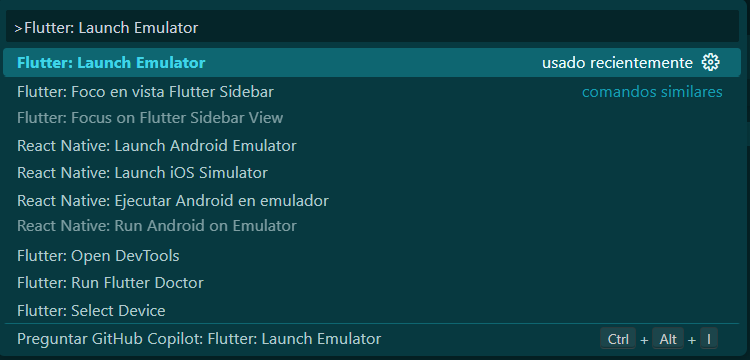
\includegraphics[width=0.9\linewidth]{img/launch_emulator.png}
    \caption{Ventana de opciones de usuario}
    \label{fig:launch_emulator}
\end{figure}

Seleccionando la opción anterior, se desplegará una lista con los emuladores disponibles, donde debería de aparecer el emulador creado anteriormente.
\begin{figure}[H]
    \centering
    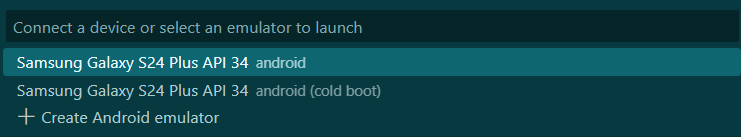
\includegraphics[width=0.9\linewidth]{img/lista_emuladores.png}
    \caption{Lista con todos los emuladores disponibles}
    \label{fig:lista_emuladores}
\end{figure}

Se iniciará el emulador, y el último paso es lanzar la aplicación con el siguiente comando.
\begin{verbatim}
    flutter run
\end{verbatim}